%---------------------------------------------------------------------
%
%                          Contribuciones
%
%---------------------------------------------------------------------

\chapter{Videojuegos de ejemplo}

Durante el proceso de desarrollo de nuestro motor de videojuegos y editor, hemos tenido la oportunidad de aplicar estas herramientas en la creaci�n de varios videojuegos. Estos proyectos nos han permitido poner a prueba el potencial y la versatilidad de nuestro motor, as� como demostrar su capacidad para crear una variedad de experiencias de juego. A continuaci�n, destacamos algunos de los videojuegos que hemos desarrollado utilizando nuestras propias herramientas:

\section{Space Invaders}

Uno de nuestros primeros proyectos fue una versi�n simplificada del juego Space Invaders, este juego nos permiti� poner a prueba cosas como los cambios de escenas, instanciacion de prefabs, manejo del input del jugador y las colisiones a trav�s del scripting. 

\medskip

En la imagen \ref{fig:spaceInvaders} se puede observar una captura del juego.


\begin{figure}[h]
    \centering
    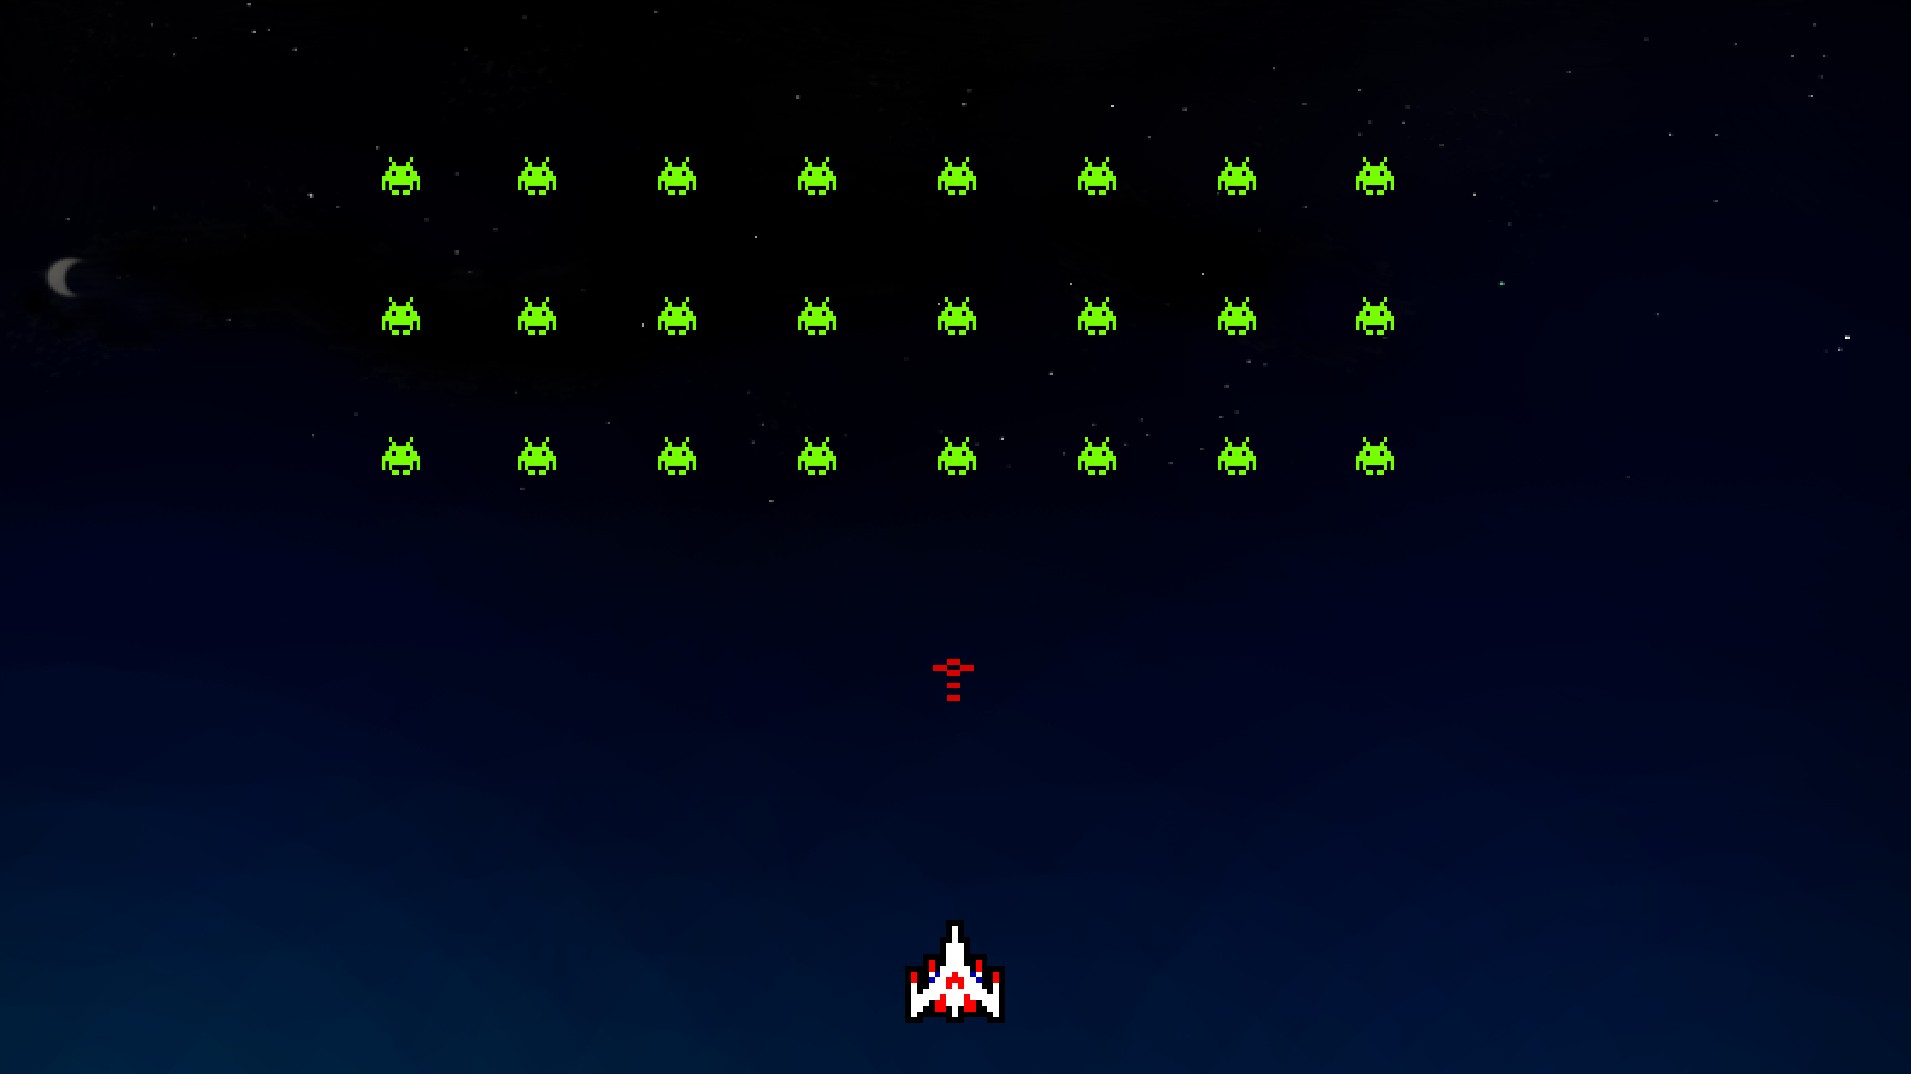
\includegraphics[width=0.6\textwidth]{Imagenes/Vectorial/SpaceInvaders.png}
    \caption{Space Invaders desarrollado con ShyEngine.}
    \label{fig:spaceInvaders}
\end{figure}

\section{Plataformas gen�rico}

Tambi�n hemos desarrollado un peque�o juego de plataformas que nos permiti� usar animaciones, sistema de part�culas y un movimiento de plataformeo.

\medskip

En la imagen \ref{fig:plataformeo} se puede observar una captura del juego.

\begin{figure}[h]
    \centering
    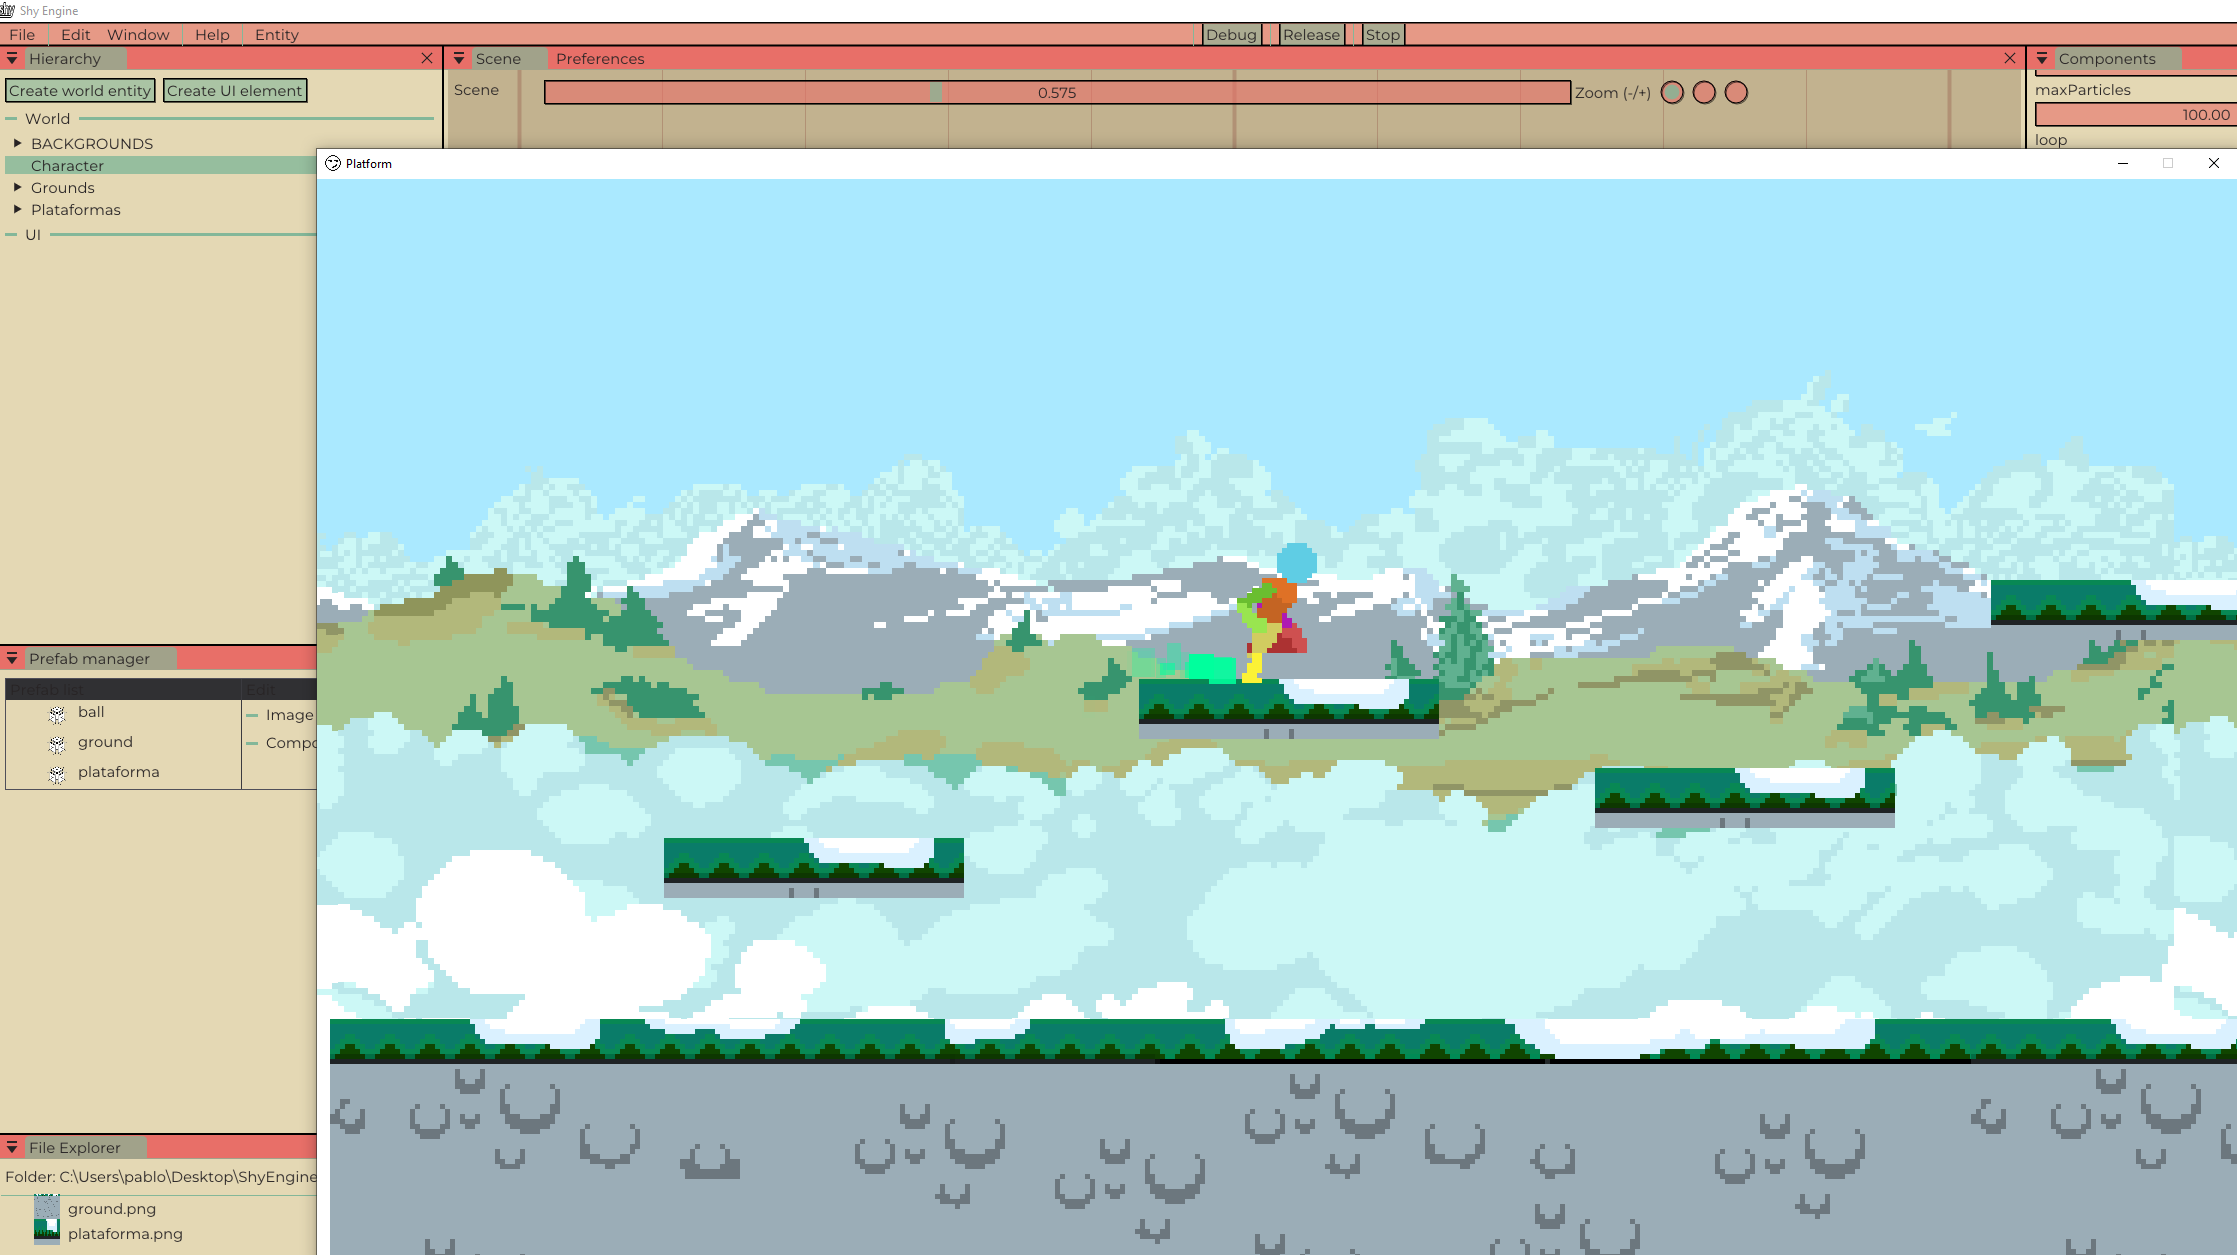
\includegraphics[width=0.6\textwidth]{Imagenes/Vectorial/Plataformas.png}
    \caption{Juego de plataformas gen�rico desarrollado con ShyEngine.}
    \label{fig:plataformeo}
\end{figure}